% RACER-GT methodology manuscript (Traditional Chinese).
% Build:  python scripts/build_docs.py --only methodology --lang zh
% Shared font, package and theorem setup lives in _preamble-zh.tex.
\documentclass[12pt,a4paper,oneside]{article}
% Traditional Chinese setup. Compile with XeLaTeX.
\usepackage{fontspec}
\usepackage{xeCJK}
\setmainfont{Noto Serif}
\setsansfont{Noto Sans}
\setmonofont{Noto Sans Mono}
\setCJKmainfont{Noto Serif CJK TC}
\setCJKsansfont{Noto Sans CJK TC}
\setCJKmonofont{Noto Sans CJK TC}
\XeTeXlinebreaklocale "zh"
\XeTeXlinebreakskip = 0pt plus 1pt

% Single source of truth for version and date across every RACER-GT document.
% Regenerate nothing by hand: bump here, rebuild, and every PDF agrees.
\newcommand{\racerversion}{1.1.0}
\newcommand{\racerdate}{2026-07-27}
\newcommand{\racerauthor}{Yi-Hao Lai}
\newcommand{\raceraffil}{Department of Finance, Da-Yeh University}
\newcommand{\raceremail}{yhlai@mail.dyu.edu.tw}
\newcommand{\racerrepo}{https://github.com/yhlai0911/RACER-GT}

% Shared package set and mathematical macros for every RACER-GT document,
% in both languages. Language-specific font and theorem-name setup lives in
% _preamble-zh.tex and _preamble-en.tex.
%
% Font policy: the build depends only on the five Noto families below. They are
% installable on Linux CI (fonts-noto-core, fonts-noto-cjk) and on macOS via
% Homebrew casks. Do not introduce a font outside this set without adding it to
% .github/workflows/docs.yml as well, or the PDF build stops being reproducible.

\usepackage[margin=2.35cm,headheight=15pt]{geometry}
\usepackage{amsmath,amssymb,amsthm,mathtools,bm}
\usepackage{booktabs,longtable,tabularx,array,multirow}
\usepackage{graphicx,float,caption,subcaption}
\usepackage{enumitem}
\usepackage{xcolor}
\usepackage{microtype}
\usepackage{setspace}
\usepackage{fancyhdr}
\usepackage{hyperref}
\usepackage[nameinlink,noabbrev]{cleveref}
\usepackage{algorithm}
\usepackage{algpseudocode}
\usepackage{listings}
\usepackage{tikz}
\usetikzlibrary{arrows.meta,positioning,shapes.geometric,fit,calc}

\hypersetup{
  colorlinks=true,
  linkcolor=black,
  citecolor=black,
  urlcolor=blue,
  pdfauthor={\racerauthor}
}

\pagestyle{fancy}
\fancyhf{}
\rhead{v\racerversion}
\cfoot{\thepage}
\setstretch{1.28}
\setlength{\parskip}{0.35em}
\setlist[itemize]{leftmargin=2em,itemsep=0.25em,topsep=0.3em}
\setlist[enumerate]{leftmargin=2.2em,itemsep=0.25em,topsep=0.3em}

% ---------------------------------------------------------------- mathematics
\newcommand{\E}{\mathbb{E}}
\newcommand{\Var}{\operatorname{Var}}
\newcommand{\Cov}{\operatorname{Cov}}
\newcommand{\tr}{\operatorname{tr}}
\newcommand{\diag}{\operatorname{diag}}
\newcommand{\argmin}{\operatorname*{arg\,min}}
\newcommand{\argmax}{\operatorname*{arg\,max}}
\newcommand{\one}{\bm{1}}
\newcommand{\Rset}{\mathbb{R}}
\newcommand{\R}{\mathbb{R}}
\newcommand{\plim}{\operatorname*{plim}}
\newcommand{\RACER}{\textsc{Racer-GT}}
\newcommand{\indic}[1]{\mathbb{I}\!\left\{#1\right\}}
\newcommand{\Sig}{\bm{\Sigma}}
\newcommand{\wvec}{\bm{w}}
\newcommand{\evec}{\bm{e}}
\newcommand{\Zvec}{\bm{Z}}

% Design facets, used identically in both languages so that a reader can move
% between the Chinese and English documents without re-learning notation.
\newcommand{\facetT}{\mathcal{T}}   % historical date
\newcommand{\facetD}{\mathcal{D}}   % collection day
\newcommand{\facetS}{\mathcal{S}}   % collection stream
\newcommand{\facetR}{\mathcal{R}}   % technical replicate

\lstset{
  basicstyle=\ttfamily\footnotesize,
  breaklines=true,
  frame=single,
  rulecolor=\color{gray!40},
  backgroundcolor=\color{gray!5},
  columns=fullflexible,
  keepspaces=true,
  showstringspaces=false
}


\setlength{\parindent}{2em}

\newtheorem{assumption}{假設}[section]
\newtheorem{proposition}{命題}[section]
\newtheorem{corollary}{推論}[section]
\newtheorem{remark}{說明}[section]
\newtheorem{definition}{定義}[section]
\newtheorem{lemma}{引理}[section]

\renewcommand{\proofname}{證明}
\renewcommand{\abstractname}{摘要}
\renewcommand{\contentsname}{目錄}
\renewcommand{\refname}{參考文獻}
\renewcommand{\tablename}{表}
\renewcommand{\figurename}{圖}

\crefname{assumption}{假設}{假設}
\crefname{proposition}{命題}{命題}
\crefname{corollary}{推論}{推論}
\crefname{definition}{定義}{定義}
\crefname{lemma}{引理}{引理}
\crefname{equation}{式}{式}
\crefname{table}{表}{表}
\crefname{figure}{圖}{圖}
\crefname{section}{節}{節}

\lhead{RACER-GT 方法論與技術報告}

\title{\bfseries
RACER-GT：在重複抽樣、分段正規化與相依量測下\\
建構長期日頻 Google Trends 指標\\[0.5em]
\large 實驗設計、全域重疊圖校準、廣義信度理論與共變異數調整估計
}
\author{Yi-Hao Lai and RACER-GT contributors\\
\small 方法論與軟體技術報告，版本 1.0.0}
\date{2026 年 7 月 27 日}

\begin{document}
\maketitle

\begin{abstract}
Google Trends（GT）已廣泛用作投資人注意力、資訊需求與情緒的高頻代理變數；然而，網站版 GT 的每次請求會重新縮放為 0--100，長期日頻資料往往必須切割為多個短視窗，且在相同查詢設定下重複下載仍可能出現不同數值。若研究者只下載一次、逐段接合後直接投入財金模型，分段尺度誤差、重複量測相依性、低搜尋量的零值與四捨五入，以及下游解釋變數的 measurement-error attenuation，均可能扭曲估計與預測結論。

本文提出 \RACER（Randomized Acquisition, Calibration, Error Decomposition, and Reliability for Google Trends），其核心不是宣稱能恢復 Google 的絕對搜尋次數，而是先明確定義兩個可識別的統計目標：固定查詢與取得設計下的 GT 期望回傳值，以及共同尺度下的潛在相對搜尋訊號。方法依序結合：（一）可預先註冊的平衡重複取得實驗與 protocol hash；（二）使用所有重疊區間的全域圖形加權最小平方法，以避免 sequential stitching 的誤差累積；（三）完整保留 exact duplicates，並以去除共同訊號後的殘差建立 near-duplicate dependence graph；（四）將 historical date、collection day、collection stream 與 technical replicate 視為交叉 facets 的 Generalizability Theory；（五）以誤差共變異數調整的 GLS／穩定化最小變異凸組合重建日頻共識；（六）以週頻與月頻資料進行二次規劃式 temporal benchmarking；（七）分離 detection、level 與 daily-innovation reliability；以及（八）將日頻 GT 的測量不確定性傳遞至下游 reliability-corrected OLS 與 SIMEX。

本文給出識別條件、無偏性與最小變異性之條件式證明、完整 decision tree，以及 Python 套件實作。20 次受控 Monte Carlo 顯示，在本文設定的資料生成過程中，\RACER 的平均 RMSE 為 3.5265，低於單一 pull 的 7.2305、跨 pull 中位數的 4.1710 與簡單平均的 3.7253。這些結果支持該框架能在特定條件下降低重建均方誤差，但不構成對所有關鍵字、地區與 GT 版本的普遍最優保證。

\noindent\textbf{關鍵詞：}Google Trends；投資人注意力；測量誤差；實驗設計；Generalizability Theory；圖形校準；GLS；temporal benchmarking；SIMEX
\end{abstract}

\begin{center}
\begin{minipage}{0.94\textwidth}
\small
\textbf{研究定位聲明。}本文所稱「偏誤降低」與「無偏」均為相對於明確定義之 estimand，並建立在可檢驗或可敏感度分析的假設上。Google 未公開網站版 GT 的完整抽樣分配、random seed、sample ID 或伺服器配置，因此不可能僅由重複下載無條件證明其等於絕對搜尋量，也不能以不同 IP 位址直接推論樣本獨立。
\end{minipage}
\end{center}

\begingroup
\setstretch{1.0}
\setlength{\parskip}{0pt}
\small
\tableofcontents
\endgroup
\newpage

\section{研究問題與方法論動機}

Google Trends 將搜尋活動轉化為相對搜尋興趣（relative search interest）指標，因其即時性與高頻特性，已被財金研究用來衡量投資人注意力、資訊需求與恐慌情緒，例如 Da, Engelberg, and Gao（2011, 2015）以及後續的報酬、波動與交易量研究。這類資料的經濟直覺很清楚：投資人未必進行交易，但通常會在形成交易意圖或受到市場事件刺激時先搜尋資訊。因此，搜尋活動可補足交易資料只記錄已實現行為的限制。

然而，GT 的便利性也容易掩蓋其測量結構。Google 官方說明指出，Trends 使用搜尋活動的樣本，將資料依時間與地區正規化，再縮放至 0--100；低搜尋量可能呈現為零。網站版每一次請求均在該次請求的範圍內重新縮放，而 2025 年公布的 API alpha 雖提供跨請求一致尺度，歷史範圍仍為滾動約 1,800 天，且數值仍不是絕對搜尋次數 \cite{googlefaq,googleapi2025}。因此，若研究期橫跨 2010--2026 年，網站版資料通常仍需切成多個短視窗後重建。

既有研究已分別指出：GT 存在 sampling noise 與 frequency inconsistency \cite{eichenauer2022}；不同時間下載相同查詢可能產生不一致結果 \cite{cebrian2024,medeiros2021}；低量關鍵字在 0--100 整數尺度下會遭受嚴重 rounding 與 censoring，因而需要 anchor calibration \cite{west2020}；長期高頻資料可利用重疊視窗進行 knitting \cite{bleher2022}。然而，若研究目的不只是在資料層面平滑一條曲線，而是要讓其進入財金計量模型，仍需同時回答下列問題：

\begin{enumerate}
  \item 重複下載的 estimand 是什麼？「真實搜尋次數」是否可識別？
  \item 如何以實驗設計控制 collection day、stream、request order 與 technical replicate？
  \item 每一個 complete pull 內，各自被正規化的 chunks 如何放到共同尺度？
  \item exact duplicates、near duplicates 與一般 sampling variation 應如何區分，而不進行 outcome-guided deletion？
  \item 如何以 ANOVA／G-theory 分解誤差來源，並決定增加 days、streams 或 replicates 哪一項最有效？
  \item 若 pulls 相互依賴，如何避免把 21 次下載錯當成 21 份獨立資訊？
  \item 如何使日頻形狀與較可靠的週頻、月頻長期尺度一致？
  \item GT 作為財金模型解釋變數時，如何修正 measurement-error attenuation？
\end{enumerate}

\RACER 將上述問題整合為一條從資料取得到下游推論的可重現測量鏈。其流程如\cref{fig:workflow}。

\begin{figure}[H]
\centering
\begin{tikzpicture}[
  node distance=7mm and 8mm,
  box/.style={rectangle, rounded corners, draw=black, align=center, minimum height=9mm, text width=3.65cm, inner sep=4pt},
  arrow/.style={-{Latex[length=2.2mm]}, thick}
]
\node[box] (estimand) {1. 定義 estimand 與鎖定 query protocol};
\node[box, right=of estimand] (design) {2. 平衡 collection-day $\times$ stream $\times$ replicate 設計};
\node[box, right=of design] (audit) {3. Raw response 保存、hash 與 protocol audit};
\node[box, below=of audit] (graph) {4. 每個 pull 的全域 overlap-graph calibration};
\node[box, left=of graph] (dup) {5. Exact audit 與 residual near-duplicate graph};
\node[box, left=of dup] (gstudy) {6. Level / detection / innovation G-study};
\node[box, below=of gstudy] (gls) {7. Covariance-adjusted GLS consensus};
\node[box, right=of gls] (bench) {8. Weekly / monthly temporal benchmarking};
\node[box, right=of bench] (decision) {9. Locked decision tree 與 uncertainty output};
\node[box, below=of decision] (eiv) {10. Downstream EIV correction / SIMEX};
\draw[arrow] (estimand) -- (design);
\draw[arrow] (design) -- (audit);
\draw[arrow] (audit) -- (graph);
\draw[arrow] (graph) -- (dup);
\draw[arrow] (dup) -- (gstudy);
\draw[arrow] (gstudy) -- (gls);
\draw[arrow] (gls) -- (bench);
\draw[arrow] (bench) -- (decision);
\draw[arrow] (decision) -- (eiv);
\end{tikzpicture}
\caption{RACER-GT 的完整估計鏈。每一層均保留輸入、輸出與稽核紀錄；非相同 pulls 不因偏離中位數而被刪除。}
\label{fig:workflow}
\end{figure}

\section{統計目標、不可識別性與可證明範圍}

\subsection{三個不同的研究目標}

令 $Q$ 表示已鎖定的 query specification，包括 term/topic、geo、category、search property、語言、固定歷史起訖日與 chunk manifest。令 $R$ 表示 retrieval environment 與執行條件，例如 collection day、stream、time slot、request order、session state 以及網站端未被研究者觀察的抽樣狀態。網站版 GT 對歷史日 $t$ 的回傳可抽象寫為
\begin{equation}
Y_t(Q,R)=\mathcal{N}_{Q,R}\!\left\{S_t(Q,R)\right\},
\label{eq:gtabstract}
\end{equation}
其中 $S_t$ 為 proprietary sampling 與 aggregation 後的搜尋訊號，$\mathcal{N}_{Q,R}$ 包含 window-specific normalization、0--100 scaling、rounding、thresholding 與可能的統計處理。

本文區分三個 estimands。

\begin{definition}[絕對搜尋量]
$A_t(Q)$ 為符合查詢構念的 Google 絕對搜尋次數。網站版 GT 不直接觀察 $A_t(Q)$。
\end{definition}

\begin{definition}[GT 設計期望]
在預先定義的 retrieval distribution $\mathcal{R}$ 下，
\begin{equation}
\theta_t(Q;\mathcal{R})
=\E_{R\sim\mathcal{R}}\left[Y_t(Q,R)\right].
\label{eq:designestimand}
\end{equation}
此 estimand 描述固定 query protocol 下 GT 系統的期望回傳值。
\end{definition}

\begin{definition}[共同尺度潛在相對訊號]
令 $X_t$ 為在明確基準期 $\mathcal{B}$ 下識別的相對搜尋指標，滿足
\begin{equation}
\frac{1}{|\mathcal{B}|}\sum_{t\in\mathcal{B}}X_t=100.
\label{eq:baselineidentification}
\end{equation}
$X_t$ 不代表絕對搜尋次數，而是不同 chunks 與 pulls 在校準後共享的相對尺度。
\end{definition}

\subsection{絕對搜尋量不可由網站版 GT 單獨識別}

\begin{proposition}[絕對尺度不可識別]
假設網站版 GT 僅觀察某一 window $W$ 內經比例正規化的值
\begin{equation}
Y_t=100\frac{A_t}{\max_{\tau\in W}A_\tau},\qquad t\in W,
\end{equation}
忽略 rounding 時，對任何常數 $c>0$，序列 $A_t$ 與 $cA_t$ 產生完全相同的 $Y_t$。因此，沒有外部 anchor 或絕對量資訊時，$A_t$ 的絕對尺度不可識別。
\end{proposition}

\begin{proof}
將 $A_t$ 替換為 $cA_t$，則
\[
100\frac{cA_t}{\max_{\tau\in W}cA_\tau}
=100\frac{cA_t}{c\max_{\tau\in W}A_\tau}
=Y_t.
\]
因此資料對所有 $c>0$ 都具有相同 likelihood／observation mapping，絕對尺度無法由 $Y_t$ 唯一決定。
\end{proof}

這項結果界定了研究主張的上限：我們可以改善相對訊號的尺度一致性、降低重建誤差並量化可靠度，但不能把統計校準誤稱為「恢復真實搜尋次數」。

\subsection{設計式無偏性}

令 $R_1,\ldots,R_m$ 由預先鎖定的 $\mathcal{R}$ 產生，並考慮
\begin{equation}
\bar Y_t=\frac{1}{m}\sum_{i=1}^{m}Y_t(Q,R_i).
\end{equation}

\begin{proposition}[對 GT 設計期望的無偏性]
若 $R_i$ 具有相同邊際分配 $\mathcal{R}$，則無論 pulls 之間是否獨立，
\begin{equation}
\E(\bar Y_t)=\theta_t(Q;\mathcal{R}).
\end{equation}
獨立性只影響 $\Var(\bar Y_t)$，不影響此平均的期望。
\end{proposition}

\begin{proof}
利用期望的線性性：
\[
\E(\bar Y_t)=\frac{1}{m}\sum_{i=1}^{m}\E\{Y_t(Q,R_i)\}
=\frac{1}{m}\sum_{i=1}^{m}\theta_t=\theta_t.
\]
此推導不需 $R_i$ 相互獨立。
\end{proof}

\begin{remark}
若取得設計不是由一個明確且固定的 $\mathcal{R}$ 產生，例如 Day 30 使用擴張到「當日」的歷史終點，則每一 pull 的 estimand 不同，平均值不再對單一 $\theta_t$ 無偏。這也是固定 historical end date 的理論理由。
\end{remark}

實際的 RACER-GT 蒐集通常採分層且平衡的 day $\times$ stream $\times$ replicate 設計，而非假設所有 pulls 具有完全相同的條件分配。令 $h\in\mathcal{H}$ 表示預先鎖定的 design cell，$\pi_h$ 為研究者事先指定的目標權重，且
\begin{equation}
\theta_{th}=\E(Y_{thi}\mid H=h),
\qquad
\theta_t^{\pi}=\sum_{h\in\mathcal{H}}\pi_h\theta_{th},
\qquad \sum_h\pi_h=1.
\label{eq:stratifiedestimand}
\end{equation}
若 cell $h$ 完成 $n_h$ 次有效重複量測，定義
\begin{equation}
\widehat\theta_t^{\pi}
=\sum_{h\in\mathcal{H}}\pi_h\bar Y_{th},
\qquad
\bar Y_{th}=\frac{1}{n_h}\sum_{i=1}^{n_h}Y_{thi}.
\label{eq:stratifiedestimator}
\end{equation}

\begin{proposition}[分層設計估計量的無偏性]
若每一 design cell 內的有效量測均以不依賴其未觀察回傳值的規則納入，且 $\E(Y_{thi}\mid H=h)=\theta_{th}$，則
\begin{equation}
\E(\widehat\theta_t^{\pi})=\theta_t^{\pi},
\end{equation}
即使同一 cell 內或不同 cells 之間的 pulls 相關，結論仍成立。相關性只改變變異數與有效資訊量。
\end{proposition}

\begin{proof}
由條件期望與線性性，
\[
\E(\widehat\theta_t^{\pi})
=\sum_h\pi_h\E(\bar Y_{th})
=\sum_h\pi_h\theta_{th}
=\theta_t^{\pi}.
\]
推導不需假設 $\Cov(Y_{thi},Y_{th'j})=0$。但若 failed requests、partial responses 或事後刪除與未觀察的 $Y_{thi}$ 有關，則 cell mean 可能產生 informative-missingness bias，故 raw audit 與預先指定排除規則不可省略。
\end{proof}

平衡設計是 $\pi_h=1/|\mathcal{H}|$ 的特例；若某些 collection days 或 streams 在目標 retrieval distribution 中應有不同權重，必須在看見資料前指定 $\pi_h$，而不是依結果調整。

\section{資料取得實驗與 protocol locking}

\subsection{交叉因素設計}

RACER-GT 將取得程序視為 repeated-measurement experiment，而非將每次下載模糊地稱為「獨立樣本」。基本設計為
\begin{equation}
D\times S\times R,
\end{equation}
其中 $D$ 為 collection-day levels、$S$ 為 collection streams、$R$ 為每個 day $\times$ stream cell 內的 technical replicates。本文建議的起始設計為 Day 0、1、2、7、14、21、30，三個固定 streams；若資源允許，$R=2$ 可將 pure technical error 與最高階交互作用分離。若僅 $R=1$，仍可估計 day 與 stream facets，但 $TDS$ 與純 replication error 無法分離。

Collection stream 應被定義為固定的複合環境：裝置、瀏覽器 profile、cookie、登入狀態、client 版本、網路與 IP 等條件在 stream 內保持不變。除非另行採用 crossover factorial design，估計出的 $S$ effect 只能稱為 composite stream effect，不能拆解為 IP effect。

為避免 stream 與 request order 或 time slot 完全混淆，RACER-GT 以 cyclic／Latin-square-like rotation 平衡每一天的 stream order；chunk order 亦可輪替。若三個 streams 無法同時啟動，這種平衡至少能使系統狀態隨時間的變化不固定落在同一個 stream。

\subsection{固定歷史窗、chunk manifest 與 protocol hash}

所有正式 pulls 必須共用：
\begin{itemize}
  \item 相同的 historical start 與 end；
  \item 相同的 chunk start/end、overlap 與 query parameters；
  \item 相同的資料清理、partial-period 排除與時區規則；
  \item 相同的 calibration、duplicate、G-study、consensus 與 decision thresholds；
  \item 相同版本的程式碼與設定檔。
\end{itemize}

設定物件以 canonical JSON 序列化並計算 SHA-256：
\begin{equation}
h=\operatorname{SHA256}\{\operatorname{canonical}(Q,\mathcal{D},\mathcal{C},\mathcal{T})\},
\end{equation}
其中 $\mathcal{D}$ 是蒐集設計，$\mathcal{C}$ 是校準設定，$\mathcal{T}$ 是 decision thresholds。每筆 raw row 可保存 $h$，若任何設定被改動，protocol hash 即改變。

\subsection{Pilot 與 confirmatory batch 的分離}

Day 0--2 的 MONITOR 可用來檢查缺漏、query drift、exact duplicates、overlap graph 是否連通與程式執行錯誤；但若研究團隊因此修改 thresholds、stitching rule、query、code 或 decision tree，Day 0--2 必須被重新標記為 pilot，正式 confirmatory batch 由新的 Day 0 開始。否則同一資料同時被用來設計與驗證規則，形成 data-dependent acceptance bias。

同理，所有 GT 處理規則都必須在查看報酬、波動、價差、VaR 或其他財金結果之前鎖定。以「哪種 GT 建構最顯著」作為資料品質決策，會將 measurement validation 變成 outcome-guided model selection。

\section{第一階段：每一 complete pull 的全域重疊圖校準}

\subsection{分段正規化模型}

令一個 complete pull 包含 $J$ 個重疊 chunks。對 chunk $j$ 中歷史日 $t$ 的正值觀察，考慮近似模型
\begin{equation}
Y_{jt}=a_j X_t\exp(\epsilon_{jt}),
\qquad a_j>0,
\label{eq:chunkmodel}
\end{equation}
其中 $a_j$ 代表該次 chunk-specific normalization scale，$X_t$ 是該 pull 內欲恢復的共同相對訊號。當 $t$ 同時存在於 chunks $j$ 與 $k$ 時，
\begin{equation}
r_{jkt}=\log Y_{jt}-\log Y_{kt}
=\ell_j-\ell_k+\nu_{jkt},
\qquad \ell_j=\log a_j,
\label{eq:edgeobservation}
\end{equation}
且 $\nu_{jkt}=\epsilon_{jt}-\epsilon_{kt}$。

由於零值不能取 log，且接近零的整數 RSV 會放大 ratio noise，RACER-GT 僅使用兩邊皆高於預先指定門檻 $c_{\min}$ 的 overlap cells 估計 edge；零值仍保留於最終數列與 detection reliability，不會被任意插補為正值。

\subsection{Robust edge estimation}

對每一可用的 chunk pair $(j,k)$，令 $\mathcal{O}_{jk}$ 為重疊日期集合。edge location $\delta_{jk}=\ell_j-\ell_k$ 以 Huber M-estimator 估計：
\begin{equation}
\widehat\delta_{jk}
=\argmin_{\delta}\sum_{t\in\mathcal{O}_{jk}}
\rho_c(r_{jkt}-\delta),
\end{equation}
其中
\begin{equation}
\rho_c(u)=
\begin{cases}
\frac{1}{2}u^2, & |u|\le c,\\
c|u|-\frac{1}{2}c^2, & |u|>c.
\end{cases}
\end{equation}
這使極端 overlap cells 不至於完全決定尺度比。套件同時估計 robust scale 與 location variance $\widehat v_{jk}$，形成 edge weight $w_{jk}=1/\max(\widehat v_{jk},v_{\min})$。

\subsection{Graph WLS 識別與估計}

建立無向圖 $G=(V,E)$：每個 chunk 是 node，每個可估 edge 是一個 overlap relation。將所有 edge equations 堆疊為
\begin{equation}
\widehat{\bm\delta}=B\bm\ell+\bm\eta,
\qquad \E(\bm\eta\mid B)=\bm 0,
\qquad \Var(\bm\eta\mid B)=\Omega,
\label{eq:graphlinear}
\end{equation}
其中 $B$ 是 oriented incidence matrix。由於只可識別相對尺度，固定一個 reference chunk $r$，令 $\ell_r=0$；刪除對應欄後得到 $B_{-r}$。估計量為
\begin{equation}
\widehat{\bm\ell}_{-r}
=(B_{-r}'WB_{-r})^{-1}B_{-r}'W\widehat{\bm\delta}.
\label{eq:graphwls}
\end{equation}

\begin{proposition}[相對尺度的識別]
固定一個 reference node 後，$\bm\ell_{-r}$ 可識別若且唯若 overlap graph $G$ 連通。此時 $B_{-r}$ 具有滿 column rank，$B_{-r}'WB_{-r}$ 對任意正定 diagonal $W$ 可逆。
\end{proposition}

\begin{proof}
圖論中，連通圖的 incidence matrix rank 為 $|V|-1$。刪除任一 node 對應欄後，$B_{-r}$ rank 為 $|V|-1$，等於其欄數。反之，若圖有 $K>1$ 個 components，incidence matrix rank 為 $|V|-K<|V|-1$，即使固定單一 reference 仍存在至少 $K-1$ 個未識別的 component-level shifts。
\end{proof}

\begin{proposition}[Graph GLS 的條件式無偏性與效率]
在\cref{eq:graphlinear}、圖連通且 $W=\Omega^{-1}$ 下，\cref{eq:graphwls} 滿足
\begin{equation}
\E(\widehat{\bm\ell}_{-r}\mid B)=\bm\ell_{-r},
\end{equation}
且為所有線性無偏估計量中的最小變異估計量。
\end{proposition}

\begin{proof}
無偏性由
\[
\E(\widehat{\bm\ell}_{-r}\mid B)
=(B'WB)^{-1}B'W\E(\widehat{\bm\delta}\mid B)
=\bm\ell_{-r}
\]
得之（為簡潔略去下標 $-r$）。效率為 Gauss--Markov theorem 的直接應用。
\end{proof}

若 $\widehat\ell_j$ 近似常態且 $\Var(\widehat\ell_j)=s_j^2$，直接使用 $\exp(-\widehat\ell_j)$ 會有 lognormal transformation bias。若校準目的為將 $Y_{jt}$ 除以 $a_j$，可採一階修正
\begin{equation}
\widehat{a_j^{-1}}_{\,bc}
=\exp\left(-\widehat\ell_j-\frac{1}{2}s_j^2\right).
\label{eq:lognormalcorrection}
\end{equation}
此修正依賴近似常態與 variance estimate，故程式允許關閉作為 sensitivity analysis。

\subsection{同日多 chunk 聚合}

校準後的 chunk observation 為
\begin{equation}
\widetilde X_{jt}=Y_{jt}\exp(-\widehat\ell_j).
\end{equation}
同一歷史日通常被多個重疊 chunks 覆蓋。RACER-GT 預設依 chunk-scale variance 進行 inverse-variance aggregation：
\begin{equation}
\widehat X^{(i)}_t
=\frac{\sum_{j\in\mathcal{J}_t}\omega_{jt}\widetilde X_{jt}}
{\sum_{j\in\mathcal{J}_t}\omega_{jt}},
\qquad
\omega_{jt}=\frac{1}{\widehat{\Var}(\widehat\ell_j)+\varepsilon}.
\end{equation}
亦可使用 median 或 Huber aggregation。最後依\cref{eq:baselineidentification} 將每個 complete pull 的基準期平均設為 100。這一步明確定義相對 index，而非宣稱恢復絕對量。

逐段 stitching 只使用相鄰 chunks，前段 edge error 會遞迴傳遞至後續所有尺度；全域圖法同時使用遠近所有重疊 edges，能以 graph cycles 觀察不一致，並輸出 normal-matrix condition number、weighted edge RMSE 與 component diagnostics。

\section{第二階段：跨 pull 相依性、duplicates 與量測可靠度}

\subsection{Exact duplicate audit}

對每一 complete pull 的 numeric vector 以固定 decimal rounding 後計算 SHA-256。完全相同的向量不應從 raw archive 消失，因其 multiplicity、collection days、streams 與 raw-response hashes 本身就是 cache／共同版本／重複執行的證據。RACER-GT 採雙層資料：
\begin{itemize}
  \item \textbf{audit set：}保留所有 nominal pulls 與 exact duplicates；
  \item \textbf{analytic unique-vector set：}在 consensus covariance estimation 中，每個完全相同向量保留一個 representative，並另存 multiplicity map。
\end{itemize}

Chunk-level duplicates 與 full-series duplicates 應分別檢查；僅看完整向量可能漏掉部分 chunks 被重複回傳的情況。

\subsection{Residual near-duplicate graph}

原始 GT pulls 都共享相同的歷史訊號，因此 raw-series correlation 本來就會非常高。若以 raw correlation 作為共同抽樣或 cache dependence 的唯一依據，容易將正常的共同訊號誤判為依賴。RACER-GT 先定義 preliminary common signal
\begin{equation}
m_t=\operatorname{median}_i Z_{it},
\end{equation}
再移除 pull-specific mean bias
\begin{equation}
b_i=\frac{1}{T}\sum_t(Z_{it}-m_t),
\qquad
e_{it}=Z_{it}-m_t-b_i.
\label{eq:residualduplicate}
\end{equation}
Near-duplicate edge 必須同時通過預先指定的 value-anchored rule，例如 raw correlation、exact-cell agreement、MAE/100、positive-day Jaccard，以及 residual correlation。Connected component 只表示成員透過 edge chain 連接，不表示 component 中每一對都相似；因此報告 density、diameter、maximum clique、articulation points、minimum within-component correlations 與 maximum MAE。

Near-duplicate graph 只作依賴診斷與 covariance 建模；除 exact numeric duplicates 外，RACER-GT 不因某 pull 偏離中位數或降低 reliability 而刪除它。

\subsection{三面向 Generalizability Theory}

令 $t=1,\ldots,T$ 為 historical dates，$d=1,\ldots,D$ 為 collection-day levels，$s=1,\ldots,S$ 為 streams，$r=1,\ldots,R$ 為 technical replicates。完全交叉隨機效果模型為
\begin{align}
Y_{tdsr}
=&\ \mu+T_t+D_d+S_s+(TD)_{td}+(TS)_{ts}+(DS)_{ds}\notag\\
&+(TDS)_{tds}+E_{tdsr}.
\label{eq:gtheorymodel}
\end{align}
各隨機成分期望為零、彼此不相關，variance components 記為
\[
\sigma_T^2,\sigma_D^2,\sigma_S^2,\sigma_{TD}^2,
\sigma_{TS}^2,\sigma_{DS}^2,\sigma_{TDS}^2,\sigma_E^2.
\]

RACER-GT 對三種轉換分別執行 G-study：
\begin{align}
\text{Level: }&\quad Y_{tdsr},\\
\text{Detection: }&\quad I(Y_{tdsr}>0),\\
\text{Innovation: }&\quad \Delta\log(1+Y_{tdsr}).
\end{align}
這樣可避免一個單一 ICC 混合「是否被偵測到」、「數值水準是否一致」與「日變化是否一致」。

對平均 $n_D$ 個 collection days、$n_S$ 個 streams 與 $n_R$ 個 replicates 的相對決策，誤差 variance 為
\begin{equation}
\sigma_\delta^2
=\frac{\sigma_{TD}^2}{n_D}
+\frac{\sigma_{TS}^2}{n_S}
+\frac{\sigma_{TDS}^2}{n_Dn_S}
+\frac{\sigma_E^2}{n_Dn_Sn_R}.
\label{eq:relativeerror}
\end{equation}
Generalizability coefficient 為
\begin{equation}
G(n_D,n_S,n_R)
=\frac{\sigma_T^2}{\sigma_T^2+\sigma_\delta^2}.
\label{eq:gcoef}
\end{equation}

若研究關心相對排名之外的絕對水準，還要加入 day、stream 與 $DS$ effects：
\begin{equation}
\sigma_\Delta^2=\sigma_\delta^2
+\frac{\sigma_D^2}{n_D}
+\frac{\sigma_S^2}{n_S}
+\frac{\sigma_{DS}^2}{n_Dn_S},
\end{equation}
\begin{equation}
\Phi(n_D,n_S,n_R)
=\frac{\sigma_T^2}{\sigma_T^2+\sigma_\Delta^2}.
\label{eq:phicoef}
\end{equation}

\subsection{Balanced ANOVA 的 method-of-moments components}

令 $a=T,b=D,c=S$，先對 $R$ replicates 取 cell mean。Balanced ANOVA 的 expected mean squares 可寫為
\begin{align}
\E(MS_{TDS})&=\sigma_E^2/R+\sigma_{TDS}^2,\\
\E(MS_{TD})&=\sigma_E^2/R+\sigma_{TDS}^2+c\sigma_{TD}^2,\\
\E(MS_{TS})&=\sigma_E^2/R+\sigma_{TDS}^2+b\sigma_{TS}^2,\\
\E(MS_{DS})&=\sigma_E^2/R+\sigma_{TDS}^2+a\sigma_{DS}^2,\\
\E(MS_T)&=\sigma_E^2/R+\sigma_{TDS}^2+c\sigma_{TD}^2+b\sigma_{TS}^2+bc\sigma_T^2,
\end{align}
並對 $D,S$ 對稱。因此 method-of-moments estimator 例如
\begin{align}
\widehat\sigma_{TD}^2&=\frac{MS_{TD}-MS_{TDS}}{c},\\
\widehat\sigma_T^2&=\frac{MS_T-MS_{TD}-MS_{TS}+MS_{TDS}}{bc}.
\end{align}
若 $R>1$，$MS_E$ 由 cell 內殘差估計，且
\begin{equation}
\widehat\sigma_{TDS}^2=MS_{TDS}-MS_E/R.
\end{equation}
若 $R=1$，$E$ 無法分離，實作將不可分部分歸入 $TDS$。負的 method-of-moments components 可報告原值並依 protocol 選擇截為零；正式推論應另用 REML sensitivity analysis。由於 historical dates 具時間相依，係數信賴區間採 moving-block bootstrap，而非把 $T$ 天當成獨立單位。

D-study 將\cref{eq:gcoef,eq:phicoef}代入不同的 $(n_D,n_S,n_R)$，直接回答「下一筆資源應投入增加日期、streams 或 technical replicates」。因此 nominal pull count 不是充分的停止規則。

\section{第三階段：共變異數調整的潛在共識數列}

\subsection{Measurement model}

將每一個 calibrated unique pull 在相同基準期重新設為平均 100，並移除 pull-specific additive bias 後，對歷史日 $t$ 寫成
\begin{equation}
\bm Z_t=\one X_t+\bm e_t,
\qquad \E(\bm e_t)=\bm 0,
\qquad \Var(\bm e_t)=\Sigma.
\label{eq:consensusmodel}
\end{equation}
$\bm Z_t$ 為 $m\times1$ vector。Near duplicates 對應 $\Sigma$ 中較高的 off-diagonal covariance；因此它們不應被簡單計為多份獨立 evidence。

考慮線性共識 $\widehat X_t=\bm w'\bm Z_t$。若 $\one'\bm w=1$，則
\begin{equation}
\E(\widehat X_t)=X_t,
\end{equation}
而 variance 為 $\bm w'\Sigma\bm w$。

\begin{proposition}[GLS 共識]
若 $\Sigma$ 正定且已知，所有滿足 $\one'\bm w=1$ 的線性無偏估計量中，
\begin{equation}
\bm w^*=\frac{\Sigma^{-1}\one}{\one'\Sigma^{-1}\one}
\label{eq:glsweights}
\end{equation}
使 $\Var(\widehat X_t)$ 最小，且
\begin{equation}
\Var(\widehat X_t)=\frac{1}{\one'\Sigma^{-1}\one}.
\end{equation}
\end{proposition}

\begin{proof}
建立 Lagrangian
\[
\mathcal{L}(\bm w,\lambda)=\bm w'\Sigma\bm w-2\lambda(\one'\bm w-1).
\]
一階條件 $2\Sigma\bm w-2\lambda\one=0$，故 $\bm w=\lambda\Sigma^{-1}\one$。代入 $\one'\bm w=1$ 得\cref{eq:glsweights}。正定 $\Sigma$ 使目標嚴格凸，因此解唯一且為全域最小值。
\end{proof}

實務上 $\Sigma$ 必須由有限歷史日的 residual matrix 估計。RACER-GT 預設使用 Ledoit--Wolf shrinkage，使 covariance 在 $m$ 相對不小或 residuals 高度共線時仍可逆。為避免 sampling error 造成負權重與極端 extrapolation，預設解下列 convex quadratic program：
\begin{equation}
\min_{\bm w}\ \bm w'\widehat\Sigma\bm w
\quad\text{s.t.}\quad
\one'\bm w=1,\quad 0\le w_i\le \bar w.
\label{eq:constrainedweights}
\end{equation}
受限解保持 sum-to-one，因此在\cref{eq:consensusmodel}下仍線性無偏；但嚴格的 unrestricted BLUE 結論只適用\cref{eq:glsweights}。權重上限是穩定化選擇，必須在 protocol 中預先鎖定。

若某日缺少少數 pulls，實作對當日可用權重重新正規化。條件式基礎標準誤為
\begin{equation}
\widehat{se}_0=\sqrt{\widehat{\bm w}'\widehat\Sigma\widehat{\bm w}}.
\end{equation}
為反映事件日可能具有較大跨 pull dispersion，1.0.0 版再以當日 absolute deviation median 相對於全期間 median 進行 bounded local multiplier。這是 pragmatic heteroskedastic adjustment，而非完整 Bayesian posterior interval；正式研究可另以 block bootstrap 重新執行全 pipeline。

\subsection{有效 pull 資訊量}

Nominal $m$ 無法反映相依性。對 residual correlation matrix $R_e$，RACER-GT 報告 spectral participation ratio
\begin{equation}
m_{\mathrm{eff}}^{\mathrm{spectral}}
=\frac{\tr(R_e)^2}{\tr(R_e^2)}.
\label{eq:spectraleff}
\end{equation}
當 residuals 相互獨立，$R_e=I_m$，故 $m_{\mathrm{eff}}=m$；當所有 residuals 完全共線，只有一個非零 eigenvalue，$m_{\mathrm{eff}}=1$。此量是資訊濃度診斷，不是對 proprietary sampling mechanism 的正式獨立樣本數證明。

另報告 Kish weight count
\begin{equation}
m_{\mathrm{eff}}^{\mathrm{Kish}}=\frac{1}{\sum_i w_i^2},
\end{equation}
用以觀察共識是否被少數 pulls 支配。

\section{第四階段：日、週、月頻率一致化}

僅以短視窗日頻 chunks 接合，可能保留日際形狀卻失去長期尺度；Eichenauer et al.（2022）稱此為 frequency inconsistency。令 preliminary daily consensus 為 $\bm z\in\R^T$，lower-frequency benchmark 為 $\bm b\in\R^K$，aggregation matrix $A$ 的第 $k$ 列對 benchmark period $k$ 內日資料給予平均權重。

RACER-GT 的 soft benchmarking estimator 定義為
\begin{equation}
\widehat{\bm x}
=\argmin_{\bm x}
(\bm x-\bm z)'Q(\bm x-\bm z)
+(A\bm x-\bm b)'W(A\bm x-\bm b),
\label{eq:softbenchmark}
\end{equation}
其中
\begin{equation}
Q=\lambda_I I+\lambda_D D_1'D_1+\lambda_R I,
\end{equation}
$D_1$ 是 first-difference matrix；$\lambda_I$ 控制對 preliminary signal 的忠實度，$\lambda_D$ 控制修正路徑的粗糙度，$W$ 通常由 benchmark standard errors 的倒數平方組成。

\begin{proposition}[Soft benchmark 的唯一解]
若 $Q$ 正定且 $W$ 半正定，\cref{eq:softbenchmark}嚴格凸，唯一解為
\begin{equation}
\widehat{\bm x}
=\bm z+(Q+A'WA)^{-1}A'W(\bm b-A\bm z).
\label{eq:softclosed}
\end{equation}
\end{proposition}

\begin{proof}
對\cref{eq:softbenchmark}取 gradient 並令其為零：
\[
Q(\bm x-\bm z)+A'W(A\bm x-\bm b)=0.
\]
整理得 $(Q+A'WA)\bm x=Q\bm z+A'W\bm b$，等價於\cref{eq:softclosed}。$Q$ 正定使 $Q+A'WA$ 正定，因此解唯一。
\end{proof}

若 benchmark 被視為無誤差硬約束，可解
\begin{equation}
\min_{\bm x}(\bm x-\bm z)'Q(\bm x-\bm z)
\quad\text{s.t.}\quad A\bm x=\bm b,
\end{equation}
其 KKT system 為
\begin{equation}
\begin{bmatrix}
Q&A'\\A&0
\end{bmatrix}
\begin{bmatrix}\bm\delta\\\bm\lambda\end{bmatrix}
=
\begin{bmatrix}0\\\bm b-A\bm z\end{bmatrix},
\qquad \widehat{\bm x}=\bm z+\bm\delta.
\end{equation}
Soft mode 更適合 GT benchmark 本身也有 sampling variation 的情況；exact mode 可作 sensitivity analysis。若 nonnegative projection 被啟用，投影後聚合等式可能略受影響，故程式會報告 projection 是否發生。

\section{可靠度指標與預先鎖定的 decision tree}

\subsection{Detection、level 與 innovation}

RACER-GT 不以一個單一相關係數概括資料品質。Detection reliability 包括 zero/nonzero agreement、positive-day Jaccard 與 Fleiss' $\kappa$；當所有觀察都屬同一類別時，$\kappa$ 不可識別，此規則標記為 not applicable，而非錯誤判 FAIL。Level reliability 包括 Pearson、Spearman、MAE/100、G 與 $\Phi$；innovation reliability 則對 $\Delta\log(1+Y)$ 計算 correlation、sign／peak overlap 與 G-study。

Exact-cell agreement 必須與 zero share 一起解讀。兩條低量序列若多數日都為零，可能得到很高 exact agreement，卻沒有足夠正值資訊；因此 decision tree 另設 maximum zero share，並檢查 positive Jaccard。

\subsection{Acceptance rules}

一個正式 batch 的 PASS 至少需滿足以下預先指定規則：
\begin{enumerate}
  \item query、historical endpoints、chunks 與 protocol hash 完整一致；
  \item 每個 complete pull 的 overlap graph 可識別且連通；
  \item unique pulls 與 spectral effective pulls 達到門檻；
  \item zero share 未超過門檻；
  \item level 與 innovation G 達到門檻；
  \item near-duplicate component 不支配全批資料；
  \item 隨 pulls 增加的 consensus convergence MAE/100 低於門檻；
  \item 若使用 benchmark，standardized benchmark RMSE 低於門檻。
\end{enumerate}

若任一 mandatory rule 明確失敗，狀態為 FAIL；若沒有失敗但有不可判定 mandatory rule，狀態為 REVIEW；全部通過才是 PASS。PASS 的意義是「允許依鎖定 protocol 建構此相對指標」，不是 construct validity、外部效度或因果識別的證明。

關鍵詞／Topic 的 construct validity 必須另行檢查：語意與語言版本、可能的非財金用途、歷史首次合理出現時間、主要 peaks 的事件對應、搜尋量是否足夠，以及不同替代 terms 的結果是否一致。測量可靠而構念錯誤的指標仍然沒有研究效度 \cite{holzl2025}。

\section{下游財金模型的 measurement-error correction}

\subsection{Attenuation bias}

令真正的注意力訊號 $X_t$ 進入財金模型
\begin{equation}
Y_{t+h}=\alpha+\beta X_t+\bm\gamma'\bm C_t+\varepsilon_{t+h},
\label{eq:downstreamtrue}
\end{equation}
但研究者觀察
\begin{equation}
W_t=X_t+u_t,
\qquad \E(u_t\mid X_t,\bm C_t,\varepsilon_{t+h})=0.
\end{equation}
在無 controls 的 classical homoskedastic case，naive OLS 滿足
\begin{equation}
\plim\widehat\beta_{\mathrm{naive}}
=\beta\frac{\sigma_X^2}{\sigma_X^2+\sigma_u^2},
\label{eq:attenuation}
\end{equation}
故係數向零衰減。

令 $M_C=I-C(C'C)^{-1}C'$ 為 controls residual-maker。若 measurement-error covariance $\Omega_u$ 已知，則
\begin{equation}
\E(W'M_CW)=X'M_CX+\tr(M_C\Omega_u).
\end{equation}
因此 moment-corrected estimator 為
\begin{equation}
\widehat\beta_{RC}
=\frac{W'M_CY}
{W'M_CW-\tr(M_C\widehat\Omega_u)}.
\label{eq:rcestimator}
\end{equation}
RACER-GT 使用每日 consensus standard error 的平方形成 diagonal $\widehat\Omega_u$，並以 Newey--West long-run variance 對 scalar moment 提供 HAC standard error。若修正後分母非正，套件拒絕估計，因為在該假設下 latent predictor variation 不足以識別 $\beta$。

\subsection{SIMEX}

當誤差標準差可估計但解析修正不穩定時，SIMEX \cite{cookstefanski1994} 對 $\lambda\ge0$ 人工加入
\begin{equation}
W_t^{(b,\lambda)}=W_t+\sqrt{\lambda}\,\widehat\sigma_{u,t}\xi_t^{(b)},
\qquad \xi_t^{(b)}\sim N(0,1),
\end{equation}
估計 $\widehat\beta(\lambda)$ 後，以二次曲線外推至 $\lambda=-1$，模擬移除 measurement error。SIMEX 對 extrapolation form 敏感，因此應與\cref{eq:rcestimator}、sample-specific pull regressions 與 full-pipeline bootstrap 並列報告，而非只選擇較顯著者。

\section{完整演算法}

\begin{algorithm}[H]
\caption{RACER-GT 長期日頻指標建構}
\label{alg:racergt}
\begin{algorithmic}[1]
\Require Locked query $Q$；balanced retrieval design；fixed chunks；raw responses；optional lower-frequency benchmark
\Ensure Final daily index、measurement uncertainty、audit trail、acceptance decision
\State Canonicalize protocol；計算 hash；產生 collection schedule 與 chunk manifest
\State 蒐集並保存所有 raw responses；記錄 day、stream、replicate、time、order、network events 與 hashes
\State Audit historical endpoints、query parameters、chunk boundaries、partial observations 與 missing chunks
\For{each complete pull $i$}
  \State 由 usable overlaps 計算 robust log-ratio edges
  \State 建立 overlap graph；若不連通依 protocol FAIL／REVIEW
  \State 解 graph WLS 取得 chunk log scales 與 covariance
  \State 校準所有 chunks；以 inverse-variance／Huber／median 聚合同日值
  \State 依固定 baseline 將 pull index 平均設為 100
\EndFor
\State 依預先指定 design-cell weights 計算 $\widehat\theta_t^{\pi}$ 作為 design-based reference
\State 保留 exact duplicate audit；建立 analytic unique-vector set
\State 由共同中位數與 pull bias 形成 residuals；建立 near-duplicate graph
\State 對 level、detection、innovation 執行 crossed-facet G-study 與 D-study
\State 估計 residual covariance $\widehat\Sigma$；解受限或無限制 GLS latent consensus
\State 計算 conditional standard errors、spectral/Kish effective counts 與 convergence path
\If{lower-frequency benchmark available}
  \State 解 soft／exact temporal benchmarking problem
\EndIf
\State 執行 locked decision tree；輸出 PASS／REVIEW／FAIL
\State 將 final index 與 uncertainty 輸入下游 EIV correction／SIMEX
\end{algorithmic}
\end{algorithm}

\section{Python 套件實作}

\subsection{設計原則}

RACER-GT 1.0.0 採 ingestion-first architecture：統計套件不內建未經官方保證的網站 scraping。網站端點、rate limits、認證與服務條款可能變動，將 retrieval client 與估計器解耦，可使研究者在官方 API、手動 CSV export 或機構核准的 collector 間替換，而不改變統計 protocol。Collector 只需輸出固定 long-format schema。

核心模組如\cref{tab:modules}。

\begin{longtable}{p{3.5cm}p{10.5cm}}
\caption{RACER-GT 1.0.0 模組}\label{tab:modules}\\
\toprule
模組 & 功能\\
\midrule
\endfirsthead
\toprule
模組 & 功能\\
\midrule
\endhead
\texttt{config.py} & Pydantic protocol schema、欄位驗證、canonical serialization 與 SHA-256 hash。\\
\texttt{design.py} & 固定 overlap windows、balanced stream/time/chunk order 與 protocol bundle。\\
\texttt{audit.py} & Historical-window drift、query drift、partial data、missing chunks 與 metadata ambiguity。\\
\texttt{overlap.py} & Huber edge estimator、graph connectivity、WLS scale solution、condition diagnostics 與 calibrated pull aggregation。\\
\texttt{duplicates.py} & Exact vector hashes、value-anchored pair metrics、residual near-duplicate graph、components/cliques/articulation diagnostics。\\
\texttt{gstudy.py} & Balanced $T\times D\times S$ ANOVA、variance components、G/$\Phi$、D-study 與 moving-block bootstrap。\\
\texttt{consensus.py} & Design-cell weighted reference、exact-collapse map、baseline rescale、Ledoit--Wolf covariance、GLS／constrained weights、effective pull counts 與 uncertainty。\\
\texttt{benchmark.py} & Sparse aggregation matrix、soft quadratic benchmark 與 exact KKT benchmark。\\
\texttt{reliability.py} & Pairwise level/innovation metrics、Fleiss kappa、day/stream dependence 與 sequential convergence。\\
\texttt{decision.py} & 可稽核的 PASS/REVIEW/FAIL decision tree。\\
\texttt{eiv.py} & Reliability-corrected OLS、HAC inference 與 quadratic SIMEX。\\
\texttt{simulation.py} & 含 latent dynamics、day/stream effects、correlated retrieval noise、chunk normalization、rounding 與 exact duplicates 的 DGP。\\
\texttt{validation.py} & Single pull、mean、median 與 RACER-GT 的 Monte Carlo 比較。\\
\texttt{pipeline.py} & End-to-end orchestrator 與完整輸出保存。\\
\texttt{cli.py} & \texttt{design}、\texttt{audit}、\texttt{run}、\texttt{simulate}、\texttt{export-stata}。\\
\bottomrule
\end{longtable}

\subsection{最小使用範例}

\begin{lstlisting}[language=Python]
import pandas as pd
from racergt import RacerGTConfig, RacerGTPipeline

config = RacerGTConfig.load_yaml("protocol.lock.yaml")
raw = pd.read_csv("raw_chunks.csv")
benchmark = pd.read_csv("benchmark.csv")

result = RacerGTPipeline(config).fit(raw, benchmark=benchmark)
result.save("results")

print(result.decision.status)
design_reference = result.design_consensus.consensus
final_gt = result.final_series
\end{lstlisting}

CLI：
\begin{lstlisting}[language=bash]
racergt design examples/config_example.yaml --out protocol_bundle \
  --anchor-date 2026-08-01
racergt audit protocol_bundle/protocol.lock.yaml raw_chunks.csv
racergt run protocol_bundle/protocol.lock.yaml raw_chunks.csv \
  --benchmark benchmark.csv --out results
\end{lstlisting}

每一次 run 產生 design-weighted reference、final latent series、calibration scales、edge residuals、duplicate groups/components、pull covariance、weights、G-study tables、reliability/convergence、benchmark fit、decision tree 與 diagnostic report。所有中間結果可供 replication，而不是只輸出一條無法稽核的平滑序列。

\section{Monte Carlo 驗證}

\subsection{資料生成過程}

本文隨套件提供可重現 simulation。基礎 latent intensity 為
\begin{align}
L_t=&\ 30+0.004t+2.5\sin(2\pi t/7)
+4\sin(2\pi t/365.25)\notag\\
&+u_t+\sum_{q=1}^{6}\operatorname{Spike}_{qt},
\end{align}
其中 $u_t=0.92u_{t-1}+\eta_t$、$\eta_t\sim N(0,1.8^2)$，並加入六個非對稱衰減事件尖峰。真實 index 依研究期平均設為 100。

對 collection day $d$ 與 stream $s$，pull-level log error 為
\begin{equation}
\zeta_{it}=a_d+b_s+0.5g_{dt}+0.5h_{it},
\end{equation}
其中 $a_d\sim N(0,0.025^2)$、$b_s\sim N(0,0.020^2)$，$g_{dt}$ 與 $h_{it}$ 分別是具持續性的 shared-day 與 idiosyncratic AR noise。每個 chunk 再加入 $N(0,0.03^2)$ multiplicative noise，並依 chunk maximum 正規化為 0--100 後四捨五入。10\% 的 nominal pulls 複製完整 latent realization 與 raw chunks，以模擬 exact cache/version duplicates。週、月 benchmark 由真實 index 的 period average 加入已知噪音產生。

Monte Carlo 使用 2024 年 366 個日資料、三個 collection days（0、1、7）、三 streams、120-day chunks、30-day steps，共 20 次 replications，seeds 1200--1219。這是程式驗證 DGP，不是對 Google proprietary mechanism 的宣稱。

\subsection{結果}

\begin{table}[H]
\centering
\caption{20 次受控 Monte Carlo 結果}
\label{tab:mc}
\begin{tabular}{lrrrrr}
\toprule
Estimator & Mean bias & Mean MAE & Mean RMSE & Corr. & Innovation corr.\\
\midrule
Single pull & 0.0000 & 5.6452 & 7.2305 & 0.9695 & 0.8869\\
Cross-pull median & -0.1464 & 3.1973 & 4.1710 & 0.9898 & 0.9556\\
Simple mean & 0.0000 & 2.8660 & 3.7253 & 0.9919 & 0.9747\\
RACER-GT & -0.1317 & 2.7017 & 3.5265 & 0.9927 & 0.9745\\
\bottomrule
\end{tabular}
\end{table}

相較 single pull，RACER-GT 的 mean RMSE 降低
\begin{equation}
1-\frac{3.5265}{7.2305}=51.2\%.
\end{equation}
相較 simple mean 降低約 5.3\%。RACER-GT 的 level correlation 最高，但 innovation correlation 與 simple mean 幾乎相同，且 simple mean 的 mean bias 接近零，主要是所有方法都以全期平均 100 正規化。這說明 RACER-GT 的優勢主要表現在跨時間點的均方重建誤差與 level fidelity，不應誇大為每一指標均嚴格支配所有基準。

\begin{figure}[H]
\centering
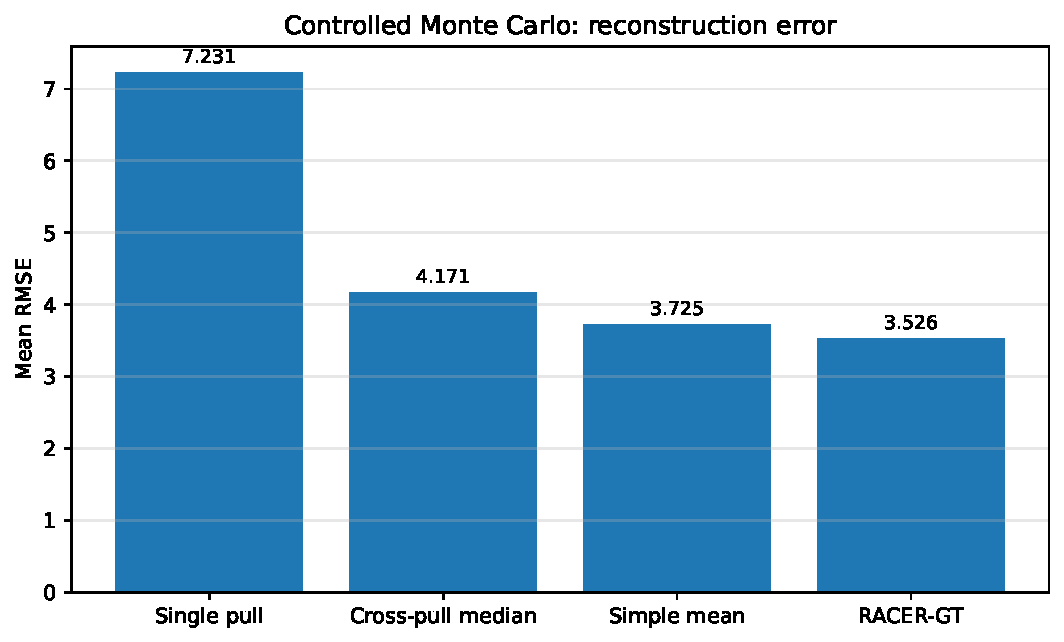
\includegraphics[width=0.78\textwidth]{figures/monte_carlo_rmse.pdf}
\caption{不同重建方法的平均 RMSE。}
\label{fig:mcrmse}
\end{figure}

\begin{figure}[H]
\centering
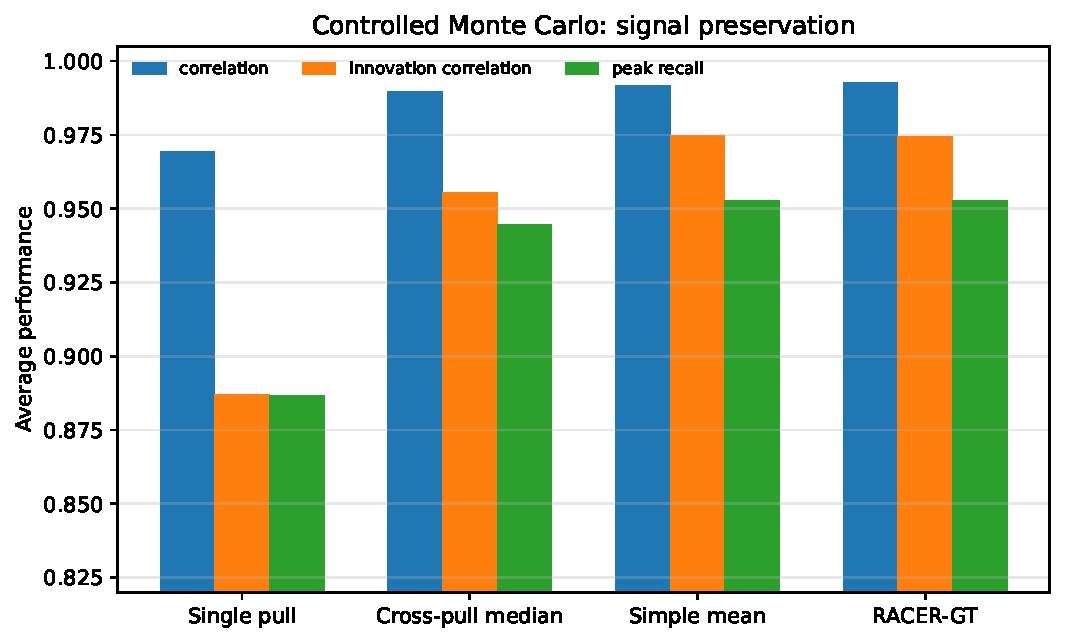
\includegraphics[width=0.82\textwidth]{figures/monte_carlo_signal.pdf}
\caption{Level correlation、innovation correlation 與 top-5\% peak recall。}
\label{fig:mcsignal}
\end{figure}

這些模擬只驗證程式在一組已知 DGP 下的行為。正式論文應針對實際關鍵字的 zero share、波動性與 sample size 重新設計 factorial Monte Carlo，至少改變：sampling noise、shared dependence、rounding/censoring、graph sparsity、structural breaks、benchmark noise、exact-duplicate fraction 與 covariance misspecification。

\section{建議的正式實驗規格}

若研究目標是 2010--2026 年單一主題的日頻 GT 指標，建議的 confirmatory protocol 如\cref{tab:recommended}。表中門檻是合理起點，不是跨研究普遍常數；應在不查看財金 outcome 的 pilot simulation 中校準，再鎖定。

\begin{longtable}{p{4.8cm}p{9.1cm}}
\caption{建議的正式 RACER-GT protocol}\label{tab:recommended}\\
\toprule
項目 & 建議設定與理由\\
\midrule
\endfirsthead
\toprule
項目 & 建議設定與理由\\
\midrule
\endhead
Historical window & 固定 2010-01-01 至明確 month-end；Day 0--30 不可使用 expanding end date。\\
Daily chunks & 先以約 180 日 window、15--30 日 step 建立密集 overlap；實際回傳頻率需程式驗證。\\
Collection days & 0、1、2、7、14、21、30，以同時觀察短期 cache/版本相似與較長期穩定度。\\
Streams & 至少三個固定 composite environments；平衡 stream order 與 time slot。\\
Replicates & 最佳為每個 day $\times$ stream 兩次，產生 42 pulls；若資源限制為 21 pulls，明確承認 pure error 不可分離。\\
Raw archive & 保存 response、numeric vectors、retrieval timestamp、query metadata、protocol hash、network events 與 client version。\\
Overlap calibration & Huber edges + global graph WLS；圖不連通原則上 FAIL，不以人工比例硬接。\\
Duplicates & Exact vectors 只在 analytic covariance 中 collapse；audit set 永久保留。Near duplicates 不刪除。\\
G-study & 分別估 level、detection、innovation；以 28-day moving-block bootstrap 估 interval。\\
Consensus & Ledoit--Wolf covariance；非負 weights；weight cap 0.5 作預設，另報 unrestricted sensitivity。\\
Frequency benchmark & 以多次擷取後的 weekly/monthly consensus 及其 SE 進行 soft benchmark；exact mode 作 robustness。\\
Stop rule & Unique count、spectral effective count、G/$\Phi$、convergence 與 component concentration 共同決定，不以 nominal 21 為充分條件。\\
Downstream model & 主結果使用 final consensus；另以 sample-specific pulls、RC-OLS、SIMEX 與 full-pipeline bootstrap 檢查。\\
\bottomrule
\end{longtable}

\section{限制、敏感度分析與可延伸方向}

\subsection{無法由統計設計消除的限制}

第一，若 Google 對所有 pulls 施加相同且隨時間變動的系統性演算法偏誤，重複量測無法僅靠平均或 GLS 識別；這是 common-mode bias。可利用 API overlap period、外部搜尋資料、新聞／交易事件與不同 query formulations 進行 external validation，但仍不是絕對真值。

第二，零值可能混合真實零搜尋、privacy threshold、sampling 與 rounding。RACER-GT 1.0.0 將零值保留並分離 detection reliability，但尚未內建 interval-censored latent count likelihood。對高 zero-share term，降為週頻、改用較廣 Topic 或 anchor-bank calibration，通常比強制製造日頻值更合理。

第三，G-theory 的 balanced method-of-moments 易於解釋，卻在 unbalanced missingness、負 variance components 或非 Gaussian binary detection 下不如 generalized linear mixed models。正式論文可將本實作作 preregistered primary estimator，再以 REML／Bayesian hierarchical model 作 robustness。

第四，benchmark 後的 1.0.0 信賴區間主要保留 cross-pull measurement uncertainty，尚未完整傳播 benchmark noise、scale calibration uncertainty 與 tuning-parameter uncertainty。最嚴謹方式是 nested moving-block bootstrap：每次重抽 historical blocks、重新估 edges、scales、duplicates、covariance、weights 與 benchmark，最後再重估財金模型。

第五，受限 GLS weights 的穩定性優於 unrestricted inverse covariance，但其最佳性取決於預先指定 constraint set。應報告 diagonal covariance、empirical covariance、Ledoit--Wolf、unrestricted GLS、equal weights 與 median 的 sensitivity table。

\subsection{必要的穩健性檢驗}

\begin{enumerate}
  \item 不同 chunk lengths、steps、positive thresholds 與 reference strategies；
  \item Huber、median 與 inverse-variance within-pull aggregation；
  \item Exact duplicate collapse 與 multiplicity-weighted sensitivity；
  \item Raw-rule、residual-rule thresholds 與 complete-linkage／maximal-clique diagnostics；
  \item G-study negative-component truncation versus REML；
  \item Consensus covariance estimators與 weight caps；
  \item Soft versus exact benchmark，不同 fidelity/smoothness weights；
  \item 最新 vintage 與多個 historical vintages；
  \item Topic versus search term、語言變體與非投資搜尋意圖排除；
  \item 財金模型中的 lag structure、UTC／市場時區、週末聚合與 publication delay。
\end{enumerate}

\subsection{與既有方法的關係}

RACER-GT 並非取代既有研究，而是把其可互補部分放入同一個測量框架。Eichenauer et al.（2022）提供 repeated draws 與 frequency consistency 的核心洞見；Bleher and Dimpfl（2022）說明高頻長期 knitting；West（2020）以 anchor bank 處理跨 query common scale 與 rounding；Cebrián and Domenech（2024）指出 repeated pulls 的誤差與熱門程度密切相關；Medeiros and Pires（2021）提醒單一 GT realization 可使 forecasting conclusion 偶然改變。RACER-GT 的新增層次在於：將 retrieval 本身明確設計為交叉測量實驗，以 graph GLS 解 within-pull scale，以 G-theory 決定蒐集資源，以 residual covariance 對相依 pulls 降權，再把 measurement uncertainty 傳至下游財金估計。

\section{結論}

長期日頻 GT 的核心問題不是「下載幾次才算獨立」，而是如何在無法觀察 proprietary sample assignment 的條件下，定義可識別 estimand、控制 retrieval design、估計分段尺度、分解誤差來源、處理相依量測，並將不確定性保留到財金模型。RACER-GT 的基本立場是：

\begin{quote}
不以 IP 取代獨立性證明；不以多數決刪除不一致 pulls；不以單一相關係數代表可靠度；不把通過資料品質決策誤稱為 construct validity；也不在下游模型中假裝建構後的 GT 沒有測量誤差。
\end{quote}

在明列假設下，全域 overlap-graph WLS 可識別相對 chunk scales；G-theory 可量化 collection day、stream 與其交互作用；GLS 可依 residual covariance 將高度相依 pulls 自動降權；temporal benchmarking 可使日頻形狀與較低頻率尺度相容；EIV correction 則能處理 GT 作為解釋變數時的 attenuation。受控模擬顯示完整方法在本文 DGP 中相較單一 pull 與簡單聚合降低 RMSE，但真正的研究價值不只是較小的某一個誤差數字，而是一套可以預先註冊、稽核、重現、否決自身資料，並誠實傳遞不確定性的測量制度。

\appendix

\section{Decision tree 的預設欄位}

\begin{longtable}{p{4.7cm}p{3.2cm}p{6.0cm}}
\toprule
Rule & 1.0.0 example & 解釋\\
\midrule
Minimum unique pulls & 12 & Exact-collapse 後的不同 numeric vectors。\\
Spectral effective pulls & 4 & 相依性調整的資訊濃度下限。\\
Maximum zero share & 0.80 & 避免資料由 threshold zeros 支配。\\
Minimum level $G$ & 0.80 & Historical-date level ranking 的重現性。\\
Minimum innovation $G$ & 0.70 & $\Delta\log(1+Y)$ 的重現性。\\
Detection $\kappa$ & 0.60 & 只有 zero/nonzero 類別有變異時適用。\\
Maximum component share & 0.50 & 避免單一 dependence component 支配。\\
Final convergence MAE/100 & 0.02 & 最後新增 pull 對 consensus 的邊際改變。\\
Benchmark standardized RMSE & 研究前校準 & 取決於 benchmark SE 與 soft constraints。\\
\bottomrule
\end{longtable}

這些值是 protocol choices，不是由統計定理產生的 universal constants。正式研究需以 pilot DGP、construct importance 與可接受 decision risk 校準。

\section{輸入資料 schema}

Raw chunk table 的必要 keys 為
\begin{lstlisting}
series_id, pull_id, chunk_id, historical_date, value,
collection_day, stream_id, replicate_id, window_start, window_end
\end{lstlisting}
強烈建議另存
\begin{lstlisting}
retrieved_at, keyword, topic_or_term, geo, category,
search_property, language, is_partial, protocol_hash,
raw_response_hash, client_version, request_order, network_event
\end{lstlisting}

\section{軟體測試與重現指令}

本版本附九組單元／整合測試，涵蓋 design、overlap calibration、duplicates/consensus、G-study、benchmark、EIV 與 full pipeline。重現：
\begin{lstlisting}[language=bash]
python -m pip install -e '.[dev]'
pytest -q
python examples/run_monte_carlo.py
\end{lstlisting}
套件亦提供 wheel、source archive、完整 README、資料字典、protocol template、Stata interoperability 與 Monte Carlo raw results。

\begin{thebibliography}{99}

\bibitem{bleher2022}
Bleher, J., \& Dimpfl, T. (2022).
Knitting multi-annual high-frequency Google Trends to predict inflation and consumption.
\textit{Econometrics and Statistics, 24}, 1--26.
\url{https://doi.org/10.1016/j.ecosta.2021.10.006}

\bibitem{brennan2001}
Brennan, R. L. (2001).
\textit{Generalizability Theory}.
Springer.

\bibitem{cebrian2024}
Cebrián, E., \& Domenech, J. (2024).
Addressing Google Trends inconsistencies.
\textit{Technological Forecasting and Social Change, 202}, 123318.
\url{https://doi.org/10.1016/j.techfore.2024.123318}

\bibitem{cookstefanski1994}
Cook, J. R., \& Stefanski, L. A. (1994).
Simulation-extrapolation estimation in parametric measurement error models.
\textit{Journal of the American Statistical Association, 89}(428), 1314--1328.
\url{https://doi.org/10.1080/01621459.1994.10476871}

\bibitem{cronbach1972}
Cronbach, L. J., Gleser, G. C., Nanda, H., \& Rajaratnam, N. (1972).
\textit{The Dependability of Behavioral Measurements: Theory of Generalizability for Scores and Profiles}.
Wiley.

\bibitem{da2011}
Da, Z., Engelberg, J., \& Gao, P. (2011).
In search of attention.
\textit{The Journal of Finance, 66}(5), 1461--1499.
\url{https://doi.org/10.1111/j.1540-6261.2011.01679.x}

\bibitem{da2015}
Da, Z., Engelberg, J., \& Gao, P. (2015).
The sum of all FEARS: Investor sentiment and asset prices.
\textit{The Review of Financial Studies, 28}(1), 1--32.
\url{https://doi.org/10.1093/rfs/hhu072}

\bibitem{denton1971}
Denton, F. T. (1971).
Adjustment of monthly or quarterly series to annual totals: An approach based on quadratic minimization.
\textit{Journal of the American Statistical Association, 66}(333), 99--102.
\url{https://doi.org/10.1080/01621459.1971.10482227}

\bibitem{eichenauer2022}
Eichenauer, V. Z., Indergand, R., Martínez, I. Z., \& Sax, C. (2022).
Obtaining consistent time series from Google Trends.
\textit{Economic Inquiry, 60}(2), 694--705.
\url{https://doi.org/10.1111/ecin.13049}

\bibitem{fuller1987}
Fuller, W. A. (1987).
\textit{Measurement Error Models}.
Wiley.

\bibitem{googleapi2025}
Google Search Central. (2025, July 24).
Introducing the Google Trends API (alpha): A new way to access Trends data.
\url{https://developers.google.com/search/blog/2025/07/trends-api}

\bibitem{googlefaq}
Google Trends Help. (n.d.).
FAQ about Google Trends data.
\url{https://support.google.com/trends/answer/4365533}

\bibitem{holzl2025}
Hölzl, J., Keusch, F., \& Sajons, C. (2025).
The (mis)use of Google Trends data in the social sciences.
\textit{Social Science Research, 126}, 103099.

\bibitem{huber1964}
Huber, P. J. (1964).
Robust estimation of a location parameter.
\textit{The Annals of Mathematical Statistics, 35}(1), 73--101.
\url{https://doi.org/10.1214/aoms/1177703732}

\bibitem{ledoitwolf2004}
Ledoit, O., \& Wolf, M. (2004).
A well-conditioned estimator for large-dimensional covariance matrices.
\textit{Journal of Multivariate Analysis, 88}(2), 365--411.
\url{https://doi.org/10.1016/S0047-259X(03)00096-4}

\bibitem{medeiros2021}
Medeiros, M. C., \& Pires, H. F. (2021).
The proper use of Google Trends in forecasting models.
\textit{arXiv:2104.03065}.
\url{https://doi.org/10.48550/arXiv.2104.03065}

\bibitem{west2020}
West, R. (2020).
Calibration of Google Trends time series.
In \textit{Proceedings of the 29th ACM International Conference on Information \& Knowledge Management} (pp. 2257--2260).
\url{https://doi.org/10.1145/3340531.3412075}

\end{thebibliography}

\end{document}
